\documentclass[compress,9pt]{beamer}
\mode<presentation>
%*******************************************************************************
% Codifica e lingua
%*******************************************************************************
\usepackage[T1]{fontenc}
\usepackage[utf8]{inputenc}
\usepackage[english,italian]{babel}

%*******************************************************************************
% Carattere
%*******************************************************************************
\usepackage{lmodern}

%*******************************************************************************
% Le solite macro
%*******************************************************************************
\newcommand{\team}{\textsf{Eta\,Beta\,Software}\xspace}
\newcommand{\customer}{\textsf{Alpha\,\&\,Partners}\xspace}
\newcommand{\inglese}[1]{\foreignlanguage{english}{#1}}
\newcommand{\tick}{\textcolor{green}{\ding{52}}}
\newcommand{\cross}{\textcolor{red}{\ding{56}}}
\newcommand{\mktg}{\foreignlanguage{english}{marketing}\xspace}
\newcommand{\sw}{\foreignlanguage{english}{software}\xspace}

%*******************************************************************************
% Tabelle
%*******************************************************************************
\usepackage{array}
\usepackage{booktabs}

%*******************************************************************************
% Immagini e multimedia
%*******************************************************************************
\graphicspath{{../pictures/}}
\usepackage{multimedia}

%*******************************************************************************
% Grafica vettoriale
%*******************************************************************************
\usepackage{tikz}
\usetikzlibrary{shadows,arrows}

%*******************************************************************************
% Pacchetti utili
%*******************************************************************************
\usepackage{pifont} % per i dingbat
\usepackage{multicol} % per dividere contenuto in più colonne
\usepackage{xspace} % per spazi condizionali
\usepackage{eurosym} % per il benedetto simbolo dell'euro

%*******************************************************************************
% Tema di beamer
%*******************************************************************************
\usetheme{JuanLesPins}
\setbeamercovered{dynamic}
\usecolortheme{orchid}

%*******************************************************************************
% Un po' di metadati
%*******************************************************************************
\title{Consulenza per software BPM}
\author{Eta Beta Software}
\date{24 luglio 2013}

% fine del preambolo e inizio del documento
\setcounter{tocdepth}{2}
\begin{document}

%*******************************************************************************
% Titolo
%*******************************************************************************
\begin{frame}
\maketitle
\end{frame}

%*******************************************************************************
% Indice
%*******************************************************************************
\begin{frame}
\begin{columns}
\column{.5\textwidth}{
\tableofcontents
}
\column{.5\textwidth}{

{\setlength{\fboxsep}{.2pt}
\rotatebox{-10}{\fbox{
\includegraphics[width=.8\textwidth]{logo}}}}

\begin{center}
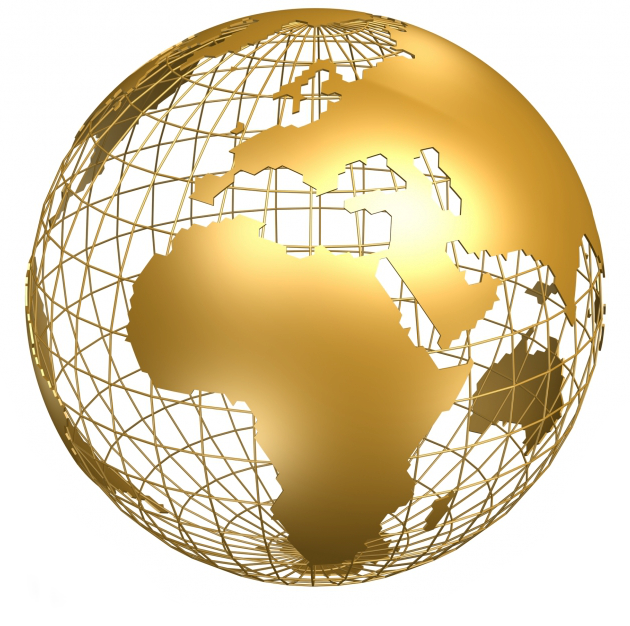
\includegraphics[width=.4\textwidth]{globe}
\end{center}


\includegraphics[width=.4\textwidth]{test}
}
\end{columns}
\end{frame}

\section{Progetto di consulenza}

\subsection{Introduzione}
\begin{frame}% #0
\frametitle{Prospettiva}
\begin{columns}
\column{.49\textwidth}{
\begin{figure}
  \centering
  \phantom{\includegraphics<2>[width=.7\textwidth]{alpha}}
  \includegraphics<1>[width=.7\textwidth]{alpha}
\end{figure}

\only<1>{
\begin{block}{Informazioni:}
  \begin{itemize}
    \item \mktg tradizionale \& digitale
    \item 2 dipendenti $+$ titolare
    \item fatturato di \EUR{200.000}
  \end{itemize}
\end{block}
}

\only<2>{
\vskip 1.25cm
\begin{flushright}
\begin{tikzpicture}
  \path[thick,red,->] (0,0) edge[bend left] ++(2, 1);
\end{tikzpicture}
\end{flushright}
}

\begin{alertblock}{Problemi:}
  Difficoltà gestione processi aziendali:
  \begin{itemize}
    \item analisi necessità clienti
    \item predisposizione offerte
    \item negoziazione e stesura proposte
  \end{itemize}
\end{alertblock}
}

\column{.49\textwidth}{
\only<1>{
\hspace{2em}
\begin{tikzpicture}
\node[inner sep=0pt] at (0, 0) {

\includegraphics[width=.6\textwidth]{postit}
};
\node[inner sep=0pt] at (.2, .1) {
\rotatebox{3}{\begin{minipage}[b]{.45\textwidth}
\scriptsize
Nel mondo l'abito\\ fa il monaco:\\ il nostro obiettivo è\\ farvi l'abito, il monaco\\ lo dovete mettere voi!
\end{minipage}
}
};
\end{tikzpicture}
}

\only<2>{
\begin{figure}
  \setlength{\fboxsep}{2pt}
  \fbox{\includegraphics<2->[width=.9\textwidth]{logo}}
\end{figure}

\begin{block}{Informazioni:}
  \begin{itemize}
    \item consulenza e sviluppo soluzioni \sw aziendali
    \item 6 dipendenti $+$ titolare
  \end{itemize}
\end{block}

\begin{center}
\begin{tikzpicture}
  \draw[thick, blue,->] (0, 1) -- (0, .5);
\end{tikzpicture}
\end{center}

\begin{exampleblock}{Soluzione:}
\begin{itemize}
  \item piano di sviluppo biennale
  \item adozione di una soluzione BPM
\end{itemize}
\end{exampleblock}
\vspace{-10pt}
}
}
\end{columns}
\end{frame}

\subsection{Pianificazione}
\subsubsection{Work Breakdown Structure}
\begin{frame}% #1
\frametitle{Scomposizione gerarchica delle attività (WBS)}
\begin{columns}
\column{.6\textwidth}{
\begin{block}{\ding{182} Pianificazione}
  \begin{enumerate}
    \item analisi di mercato e studio di fattibilità
    \item pianificazione del lavoro
    \item business plan
  \end{enumerate}
\end{block}

\begin{block}{\ding{183} Studio di Mercato}
  \begin{enumerate}
    \item analisi \sw esistenti
    \item analisi \sw prescelti
    \item valutazione soluzione ibrida / \textit{ad~hoc}
  \end{enumerate}
\end{block}

\begin{block}{\ding{184} Proposta}
  \begin{enumerate}
    \item scelta \sw
    \item redazione proposta
    \item manuale / consigli d'uso
    \item presentazione proposta
  \end{enumerate}
\end{block}
}
\column{.38\textwidth}{
\begin{figure}
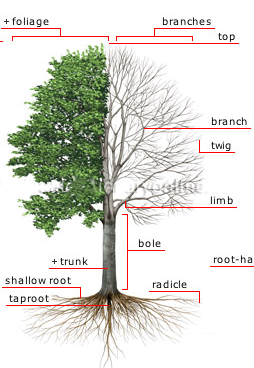
\includegraphics[width=.8\textwidth]{tree}
\end{figure}
}
\end{columns}

\end{frame}

\subsubsection{Organizational Breakdown Structure}
\begin{frame}% #2
\frametitle{Organigramma aziendale (OBS)}

\begin{tikzpicture}
\tikzstyle{every node} = [font = \sffamily\bfseries]

\node[drop shadow,fill=white,inner sep=0pt] (head) at (6, 10) {
  \begin{tabular}{|c|}
  \hline
  Titolare\\
  \hline  
  \end{tabular}
};

\node[drop shadow,fill=white,inner sep=0pt] (pm) at (4.5, 9) {
  \begin{tabular}{|c|}
  \hline
  PM\\
  \hline  
  \end{tabular}
};

\node[drop shadow,fill=white,inner sep=0pt] (admin) at (2, 9) {
  \begin{tabular}{|c|}
  \hline
  Amministratore\\
  \hline  
  \end{tabular}
};

\node[drop shadow,fill=white,inner sep=0pt] (mktg) at (7, 9) {
  \begin{tabular}{|c|}
  \hline
  Resp. MKTG\\
  \hline  
  \end{tabular}
};

\node[drop shadow, fill=white, inner sep=0pt] (qa) at (10, 9) {
  \begin{tabular}{|c|}
  \hline
  Resp. QA\\
  \hline  
  \end{tabular}
};

\node[drop shadow,fill=white,inner sep=0pt] (anal) at (4, 8) {
  \begin{tabular}{|c|}
  \hline
  Analista\\
  \hline  
  \end{tabular}
};

\node[drop shadow,fill=white,inner sep=0pt] (prog) at (8, 8) {
  \begin{tabular}{|c|}
  \hline
  Programmatore\\
  \hline  
  \end{tabular}
};

% linea di primo livello
\draw (admin.north) -- ++(0, .2) -- ++(8, 0) -- (qa.north);
\draw (pm.north) -- ++(0, .2);
\draw (mktg.north) -- ++(0, .2);
\draw (head.south) -- ++(0, -.35);

% linea di secondo livello
\draw (anal.north) -- ++(0, .2) -- ++(4, 0) -- (prog.north);
\draw (pm.south) -- ++(0, -.35);

\end{tikzpicture}

\bigskip
\pause
\begin{columns}
\column{.49\textwidth}{
\begin{alertblock}{Attenzione:}
 Risorse limitate e tempi restrittivi!
\end{alertblock}
}
\column{.49\textwidth}{
\begin{figure}
  \phantom{\includegraphics<1>[width=.6\textwidth]{hardwork}}
  \includegraphics<2->[width=.5\textwidth]{hardwork}
\end{figure}
}
\end{columns}
\end{frame}

\subsubsection{Matrice delle responsabilità}
\begin{frame}% #3
\frametitle{Intersezione fra WBS e OBS}
\begin{columns}
\column{.7\textwidth}{
\vspace{1em}
  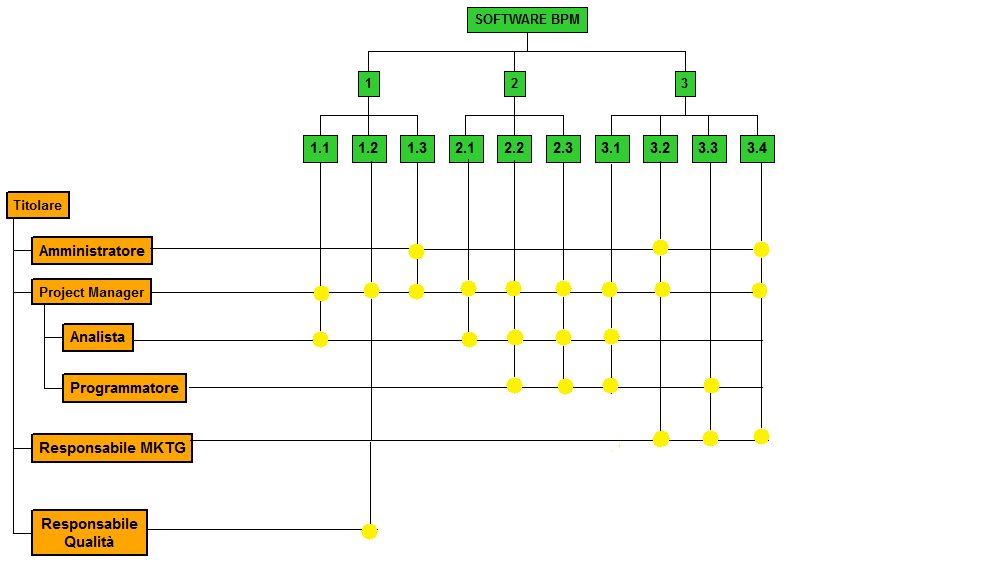
\includegraphics[width=\textwidth]{WBS_OBS}
\vfill
}
\column{.3\textwidth}{
\scalebox{.7}{
\hspace{2pt}\begin{minipage}[b]{\textwidth}
\begin{block}{\ding{182} Pianificazione}
\begin{enumerate}
  \item analisi di mercato
  \item piaificazione lavoro
  \item stesura BP
\end{enumerate}
\end{block}

\begin{block}{\ding{183} Studio di Mercato}
\begin{enumerate}
  \item analisi SW esistenti
  \item analisi SW prescelti
  \item valutazione soluzione ibrida
\end{enumerate}
\end{block}

\begin{block}{\ding{184} Proposta}
\begin{enumerate}
  \item scelta SW
  \item redazione proposta
  \item redazione manuale
  \item presentazione proposta
\end{enumerate}
\end{block}
\end{minipage}
}
}
\end{columns}
\end{frame}

%\subsubsection{Resource Breakdown Structure}
%\begin{frame} % #4
%\frametitle{Classificazione delle risorse}
%\begin{tikzpicture}
%\node at (0, 0) {
%  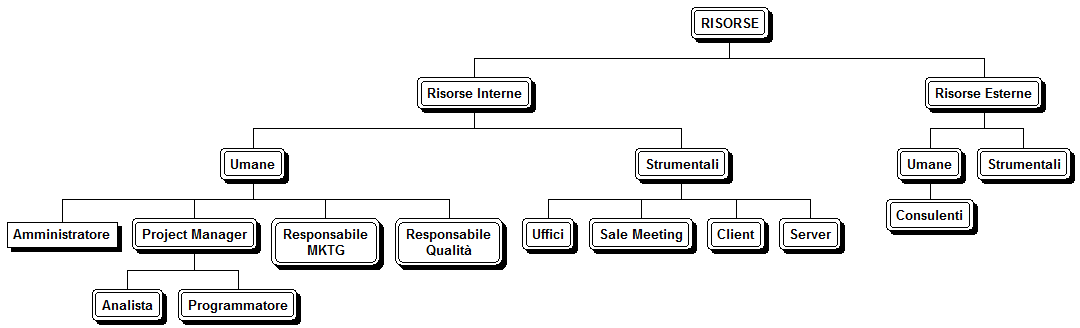
\includegraphics[width=\textwidth]{RBS}
%};

%\path[->,semithick,blue] (1.3, -2.6) edge[out=180,in=270] ++(-3, 1.2);

%\node at (2, -3) {
%\rotatebox{20}{\scalebox{.5}{
%\begin{tikzpicture}
\tikzstyle{every node} = [font = \sffamily\bfseries]

\node[drop shadow,fill=white,inner sep=0pt] (head) at (6, 10) {
  \begin{tabular}{|c|}
  \hline
  Titolare\\
  \hline  
  \end{tabular}
};

\node[drop shadow,fill=white,inner sep=0pt] (pm) at (4.5, 9) {
  \begin{tabular}{|c|}
  \hline
  PM\\
  \hline  
  \end{tabular}
};

\node[drop shadow,fill=white,inner sep=0pt] (admin) at (2, 9) {
  \begin{tabular}{|c|}
  \hline
  Amministratore\\
  \hline  
  \end{tabular}
};

\node[drop shadow,fill=white,inner sep=0pt] (mktg) at (7, 9) {
  \begin{tabular}{|c|}
  \hline
  Resp. MKTG\\
  \hline  
  \end{tabular}
};

\node[drop shadow, fill=white, inner sep=0pt] (qa) at (10, 9) {
  \begin{tabular}{|c|}
  \hline
  Resp. QA\\
  \hline  
  \end{tabular}
};

\node[drop shadow,fill=white,inner sep=0pt] (anal) at (4, 8) {
  \begin{tabular}{|c|}
  \hline
  Analista\\
  \hline  
  \end{tabular}
};

\node[drop shadow,fill=white,inner sep=0pt] (prog) at (8, 8) {
  \begin{tabular}{|c|}
  \hline
  Programmatore\\
  \hline  
  \end{tabular}
};

% linea di primo livello
\draw (admin.north) -- ++(0, .2) -- ++(8, 0) -- (qa.north);
\draw (pm.north) -- ++(0, .2);
\draw (mktg.north) -- ++(0, .2);
\draw (head.south) -- ++(0, -.35);

% linea di secondo livello
\draw (anal.north) -- ++(0, .2) -- ++(4, 0) -- (prog.north);
\draw (pm.south) -- ++(0, -.35);

\end{tikzpicture}
%}}
%};

%\node at (-3, -3.5) {
%  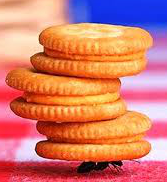
\includegraphics[width=.2\textwidth]{hardwork}
%};
%\end{tikzpicture}
%\end{frame}

\subsubsection{Pianificazione temporale}
\begin{frame}% #5
\frametitle{Diagramma di Gantt}

\begin{figure}
  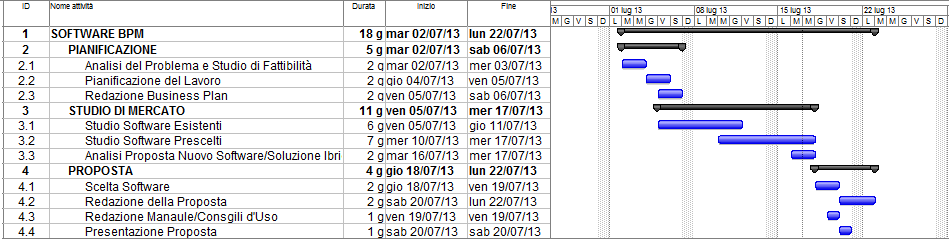
\includegraphics[width=\textwidth]{gantt}
\end{figure}

\begin{columns}
\column{.5\textwidth}{
\hspace{2em}\rotatebox{5}{
  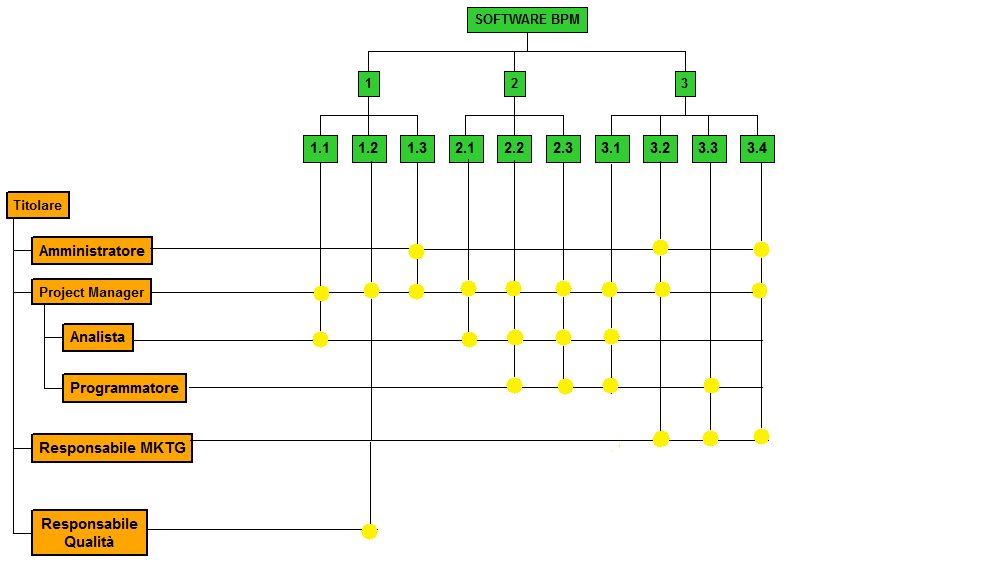
\includegraphics[width=.8\textwidth]{WBS_OBS}
}
}
\column{.5\textwidth}{
  \begin{figure}
  
\includegraphics[width=.6\textwidth]{hourglass}
  \end{figure}
}
\end{columns}
\end{frame}

\subsection{Aspetto economico}
\begin{frame}% #6
\frametitle{Preventivo dei costi}

\begin{columns}
\column{.5\textwidth}{
\scalebox{.51}{
\begin{scriptsize}
\begin{tabular}{p{.6\textwidth}ccccccr}
\toprule
\textbf{\sffamily{}Attività}& \textbf{\sffamily{}AM} & \textbf{\sffamily{}RMKTG} & \textbf{\sffamily{}PM} & \textbf{\sffamily{}RQ} & \textbf{\sffamily{}PRG} & \textbf{\sffamily{}AN} & \textbf{\sffamily{}Costo}\\
\midrule
analisi e studio di fattibilità  &   & & 5  &   & & 8 & \EUR{350,00}\\
pianificazione del lavoro                     &   & & 16 & 6 & &   & \EUR{600,00}\\
redazione \inglese{business plan}	            & 1 & & 16 &   & &   & \EUR{520,00}\\
\midrule
\scshape{}pianificazione   							      & 1 & &37 &	6 &	&	8 &	\textcolor{red}{\EUR{1.470,00}}\\
\bottomrule
\end{tabular}
\end{scriptsize}
}
}
\column{.5\textwidth}{
\scalebox{.51}{
\begin{scriptsize}
\begin{tabular}{p{.6\textwidth}ccccccr}
\toprule
\textbf{\sffamily{}Attività}& \textbf{\sffamily{}AM} & \textbf{\sffamily{}RMKTG} & \textbf{\sffamily{}PM} & \textbf{\sffamily{}RQ} & \textbf{\sffamily{}PRG} & \textbf{\sffamily{}AN} & \textbf{\sffamily{}Costo}\\
\midrule
studio software esistenti & & & 1& & 24& 23& \EUR{965,00}\\
studio software prescelti	 				  & & &	&	&40 &16 & \EUR{1.000,00}\\	
analisi nuovo SW/soluzione ibrida 					  & & &2 & 	&5	&  8  & \EUR{335,00}\\
\midrule
\scshape{}studio di mercato  							& 1 &  &3 & &69	&47	&	\textcolor{red}{\EUR{2.300,00}}\\
\bottomrule
\end{tabular}
\end{scriptsize}
}
}
\end{columns}

\bigskip

\begin{columns}
\column{.5\textwidth}{
\center
\scalebox{.51}{
\begin{scriptsize}
\begin{tabular}{p{.6\textwidth}ccccccr}
\toprule
\textbf{\sffamily{}Attività}& \textbf{\sffamily{}AM} & \textbf{\sffamily{}RMKTG} & \textbf{\sffamily{}PM} & \textbf{\sffamily{}RQ} & \textbf{\sffamily{}PRG} & \textbf{\sffamily{}AN} & \textbf{\sffamily{}Costo}\\
\midrule
scelta software			& & & 3&	& 7&	6& \EUR{345,00}\\
redazione proposta & 1&	8&	6& & & & \EUR{420,00}\\
redazione manuale / consigli d'uso & & & & & 					4 && \EUR{60,00}\\	
presentazione proposta		 & & 2&  	1	& & 	& & \EUR{80,00}\\
\midrule
\scshape{}proposta  							& 1  &10 &10& &	4&	6&	\textcolor{red}{\EUR{905,00}}\\
\bottomrule
\end{tabular}
\end{scriptsize}
}
}
\bigskip
\column{.5\textwidth}{
\scalebox{.6}{
\hspace{5em}\begin{minipage}[2]{\textwidth}
\scriptsize
\begin{tabular}{p{.6\textwidth}c}
\toprule
\textbf{\sffamily{}Ruolo}& \textbf{\sffamily{}CMO}\\
\midrule
Amministratore			  & \EUR{40,00}\\
Project Manager			  & \EUR{30,00}\\
Responsabile MKTG		  & \EUR{25,00}\\
Responsabile Qualità	& \EUR{20,00}\\
Analista				      & \EUR{25,00}\\
Programmatore		     	& \EUR{15,00}\\
Consulente				    & \EUR{30,00}\\
\bottomrule
\end{tabular}
\end{minipage}
}
}
\end{columns}

\begin{columns}
\column{.49\textwidth}{
\begin{center}
\scalebox{.6}{
\begin{scriptsize}
\begin{tabular}{p{.6\textwidth}cc}
\toprule
\textbf{\sffamily{}Attività}& \textbf{\sffamily{}Consulente} & \textbf{\sffamily{}Costo}\\
\midrule
Pianificazione		& 1 & \EUR{30,00}\\
Studio di Mercato & 5 & \EUR{150,00}\\
Proposta 			    &   &	\EUR{60,00}\\
\midrule
\scshape{}consulenza & & \textcolor{red}{\EUR{240}}\\
\bottomrule
\end{tabular}
\end{scriptsize}
}

\bigskip

\uncover<2>{
\rotatebox{10}{
\begin{tikzpicture}
\node(0,0) {
Costo totale: \textcolor{red}{\EUR{4.915}}
};
\draw[semithick,red] (0,0) circle [x radius=2, y radius=.4];
\end{tikzpicture}
}
}
\end{center}
}
\column{.49\textwidth}{
\bigskip
\begin{figure}
  
\includegraphics[width=.6\textwidth]{hourglass}
\end{figure}
}
\end{columns}
\end{frame}

\subsection{Gestione dei rischi}
\begin{frame}% #7
\frametitle{Rischi di progetto}
\begin{columns}
\column{.5\textwidth}{
\scalebox{.8}{
\begin{minipage}[b]{\textwidth}
\only<1>{
\begin{block}{Rischi legati al personale}
\begin{description}
  \item[Motivo:] impegni personali
  \item[Probabilità:] media
  \item[Impatto:] variabile
  \item[Strategia:] slack temporale
\end{description}
\end{block}
}
\only<2>{
\begin{alertblock}{Rischi legati al personale}
\begin{description}
  \item[Motivo:] impegni personali
  \item[Probabilità:] media
  \item[Impatto:] variabile
  \item[Strategia:] slack temporale
\end{description}
\end{alertblock}
}

\begin{block}{Rischi legati alla tecnologia}
\begin{description}
  \item[Motivo:] inesperienza del team
  \item[Probabilità:] alta
  \item[Impatto:] medio-grave
  \item[Strategia:] documentazione e collaborazione
\end{description}
\end{block}

\begin{block}{Rischi di mercato}
\begin{description}
  \item[Motivo:] scarse conoscenze
  \item[Probabilità:] alta
  \item[Impatto:] medio-grave
  \item[Strategia:] consulenze esterne
\end{description}
\end{block}
\end{minipage}
}
}
\column{.5\textwidth}{
\scalebox{.8}{
\begin{minipage}[b]{\textwidth}
\begin{block}{Errata stima risorse}
\begin{description}
  \item[Motivo:] inesperienza
  \item[Probabilità:] media
  \item[Impatto:] medio-grave
  \item[Strategia:] pianificazione pessimistica
\end{description}
\end{block}
\end{minipage}
}
\vfill
\begin{figure}
  
\includegraphics[width=.6\textwidth]{risk}
\end{figure}
}
\end{columns}
\end{frame}

\section{Studio di mercato}
\subsection{Software BPM}
\begin{frame}% #8
\frametitle{I software di Business Process Management}
\begin{columns}
\column{.5\textwidth}{
\hspace{4em}\rotatebox{10}{
  
\includegraphics[width=.4\textwidth]{ibm}
}\bigskip

\rotatebox{-10}{
  
\includegraphics[width=.5\textwidth]{oracle}
}\bigskip

\rotatebox{10}{
  
\includegraphics[width=.5\textwidth]{ms}
}
  
\includegraphics[width=.4\textwidth]{sap}
}
\column{.5\textwidth}{
\begin{exampleblock}{Vantaggi:}
\begin{itemize}
  \item incremento efficienza
  \item controllo coordinato e continuativo
  \item miglior pianificazione
  \item supporto decisionale
  \item dematerializzazione documenti
  \item gestione flusso informativo
\end{itemize}
\end{exampleblock}

\begin{block}{Caratteristiche:}
\begin{itemize}
  \item modellazione processi
  \item cockpit aziendale e reporting
  \item simulazione
  \item interfacciamento con servizi esterni
  \item interazione con utente (form)
  \item strumenti collaborativi
\end{itemize}
\end{block}
}
\end{columns}
\end{frame}

\subsection{Analisi delle variazioni}
\begin{frame}% #9
\frametitle{Prospettiva temporale}
\hfill\begin{minipage}[b]{.4\textwidth}
\begin{block}<2->{Situazione attuale:}
\begin{itemize}
  \item concentrazione offerta
  \item colossi come MS e Oracle
\end{itemize}
\end{block}
\end{minipage}

\begin{tikzpicture}
\node (market2000) at (0, 0) {
  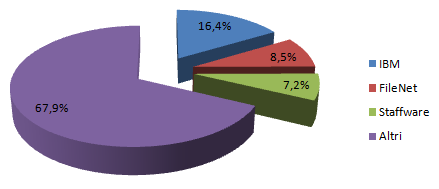
\includegraphics[width=.5\textwidth]{mercato_2000}
};
\node (market2012) at (5, -1.2) {
  \phantom{\includegraphics<1>[width=.5\textwidth]{mercato_2012}}
  \includegraphics<2->[width=.5\textwidth]{mercato_2012}
};
\path<2->[very thick,->,blue] (market2000.south) edge[bend right] (market2012.west);
\end{tikzpicture}

\begin{minipage}[b]{.4\textwidth}
\begin{block}{Situazione nel 2010:}
\begin{itemize}
  \item frammentazione
  \item piccoli fornitori
\end{itemize}
\end{block}
\end{minipage}
\end{frame}

\begin{frame}% #10
\frametitle{Analisi geotopografica}
\begin{columns}
\column{.5\textwidth}{
\begin{figure}
  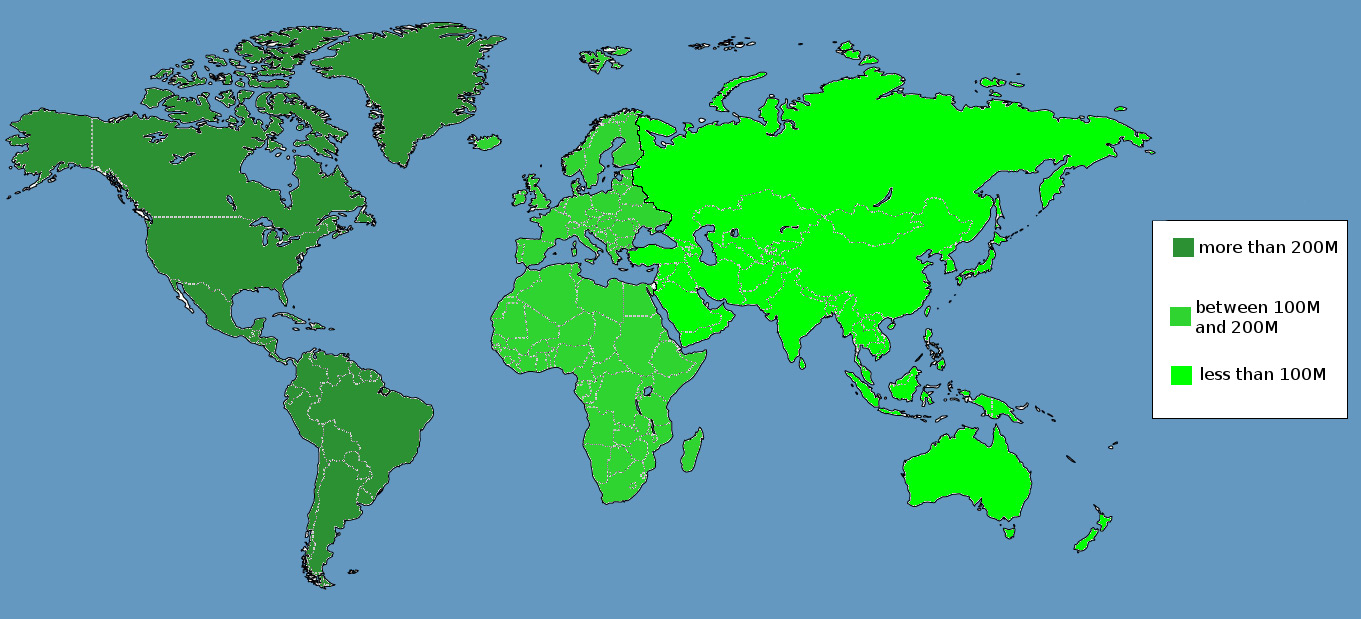
\includegraphics[width=\textwidth]{worldmap}
\end{figure}
}
\column{.5\textwidth}{
\begin{block}{America}
\begin{itemize}
  \item investimenti $\simeq$\,300\,M\,\$ nelle Americhe vs $\simeq$\,150\,M\,\$ in Europa
  \item maggior parte di fornitori oltreoceano
\end{itemize}
\end{block}
}
\end{columns}

\begin{columns}
\column{.5\textwidth}{
\uncover<2>{
\begin{block}{Europa}
\begin{itemize}
  \item crescita più elevata (+45\% annuo)
  \item potenziale emergente
\end{itemize}
\end{block}
}
}
\column{.5\textwidth}{
\only<1>{
\begin{figure}
  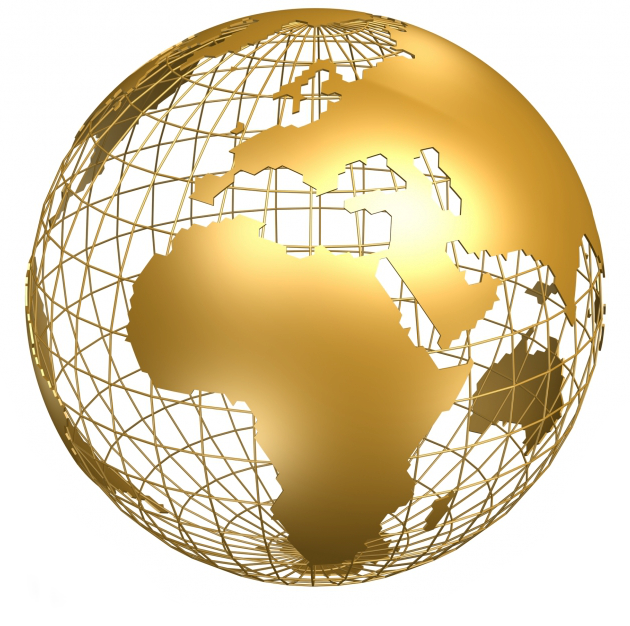
\includegraphics[width=.42\textwidth]{globe}
\end{figure}
}
\only<2>{
\begin{figure}
  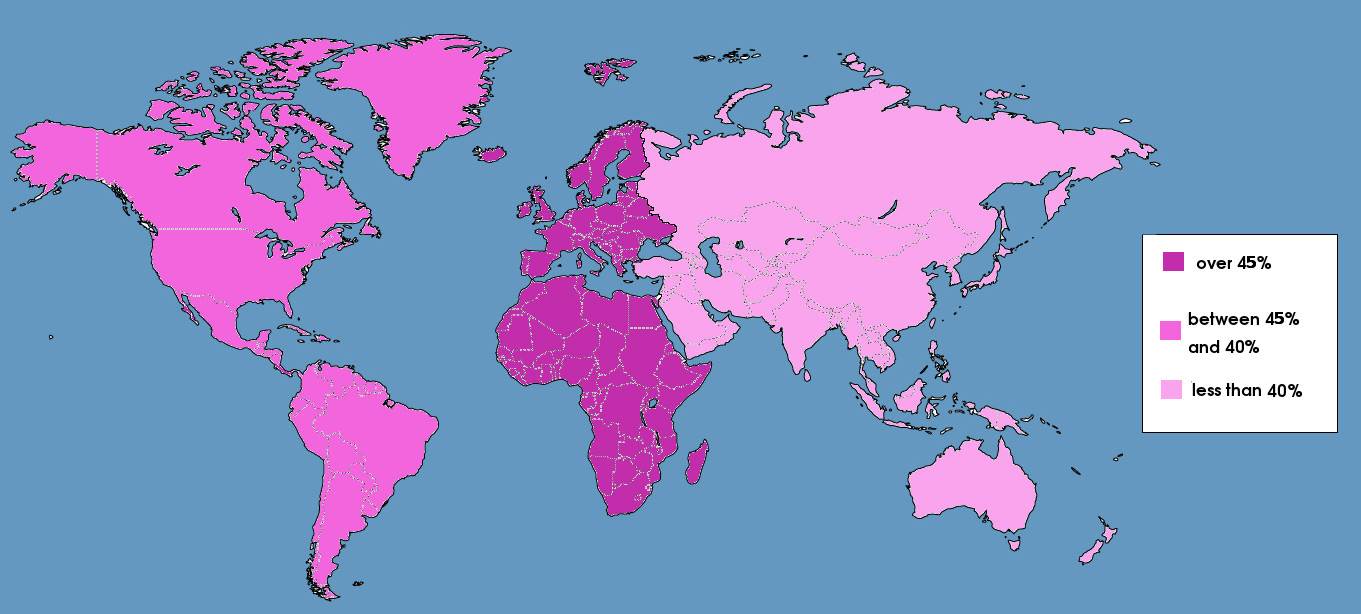
\includegraphics[width=.9\textwidth]{worldmap3}
\end{figure}
}
}
\end{columns}

\end{frame}

\section{Analisi dei \sw}
\subsection{Software selezionati}
\newcommand{\progname}{Soluzione All-in-One (BOS)}
\begin{frame}% #11
\frametitle{\progname}
\begin{columns}
\column{.5\textwidth}{
\begin{exampleblock}{\ding{52} Vantaggi:}
\begin{itemize}
  \item editor BPMN potente e intuitivo
  \item simulazione + report
  \item report + ottimizzazione
  \item interfacciamento SW di terze parti
  \item modulo Bonita XP (ruoli)
  \item Bonita Form Builder
\end{itemize}
\end{exampleblock}
}
\column{.5\textwidth}{
\begin{figure}
  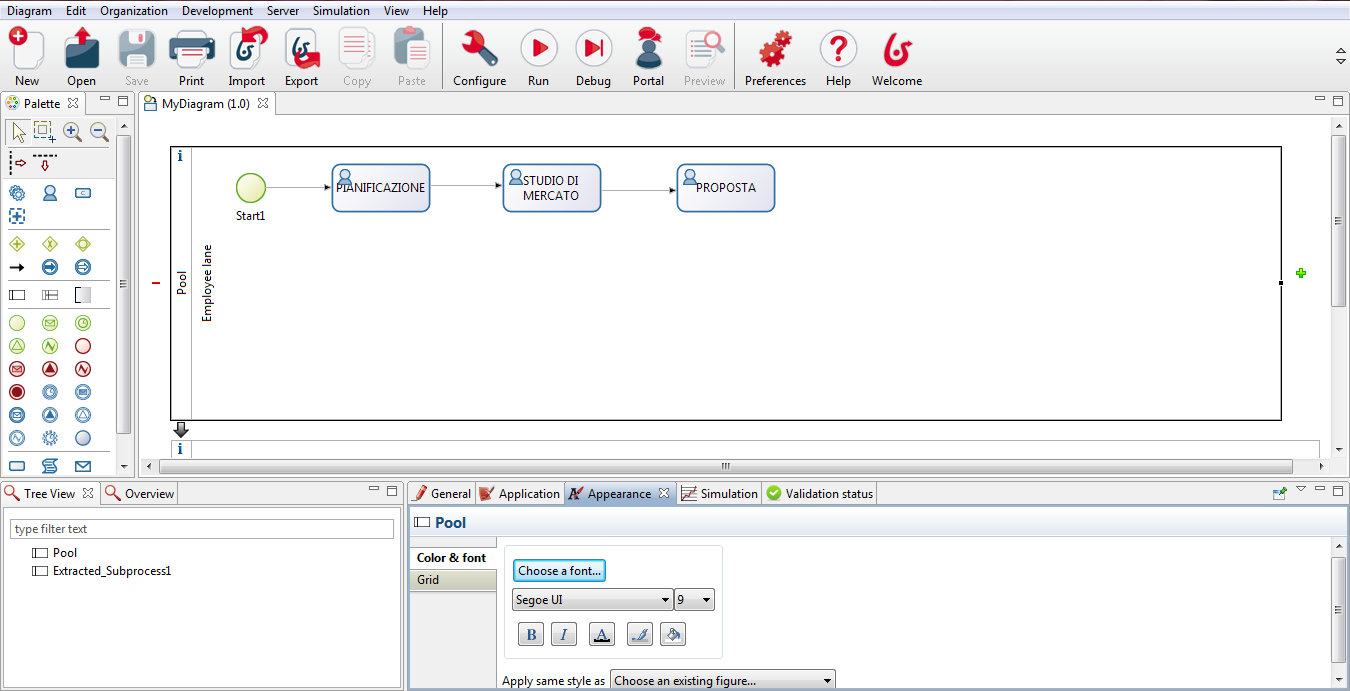
\includegraphics[width=\textwidth]{diagrammi}
\end{figure}
}
\end{columns}

\begin{columns}
\column{.5\textwidth}{
\begin{figure}
  
\includegraphics[width=.65\textwidth]{bonitasoft_logo}
\end{figure}
}
\column{.5\textwidth}{
\begin{alertblock}{\ding{56} Svantaggi:}
\begin{itemize}
  \item complessità installazione
  \item configurazione non semplice
\end{itemize}
\end{alertblock}
}
\end{columns}
\end{frame}

\renewcommand{\progname}{Bizagi}
\begin{frame}% #13
\frametitle{Una seconda soluzione (Bizagi)}
\begin{columns}
\column{.5\textwidth}{
\begin{exampleblock}{\ding{52} Vantaggi:}
\begin{itemize}
  \item editor facile da usare
  \item validazione diagrammi
  \item report esaustivo e dettagliato
  \item interfacciamento con ERP e CRM
  \item process template
  \item tool collaborativi
\end{itemize}
\end{exampleblock}
}

\column{.5\textwidth}{
\begin{figure}
  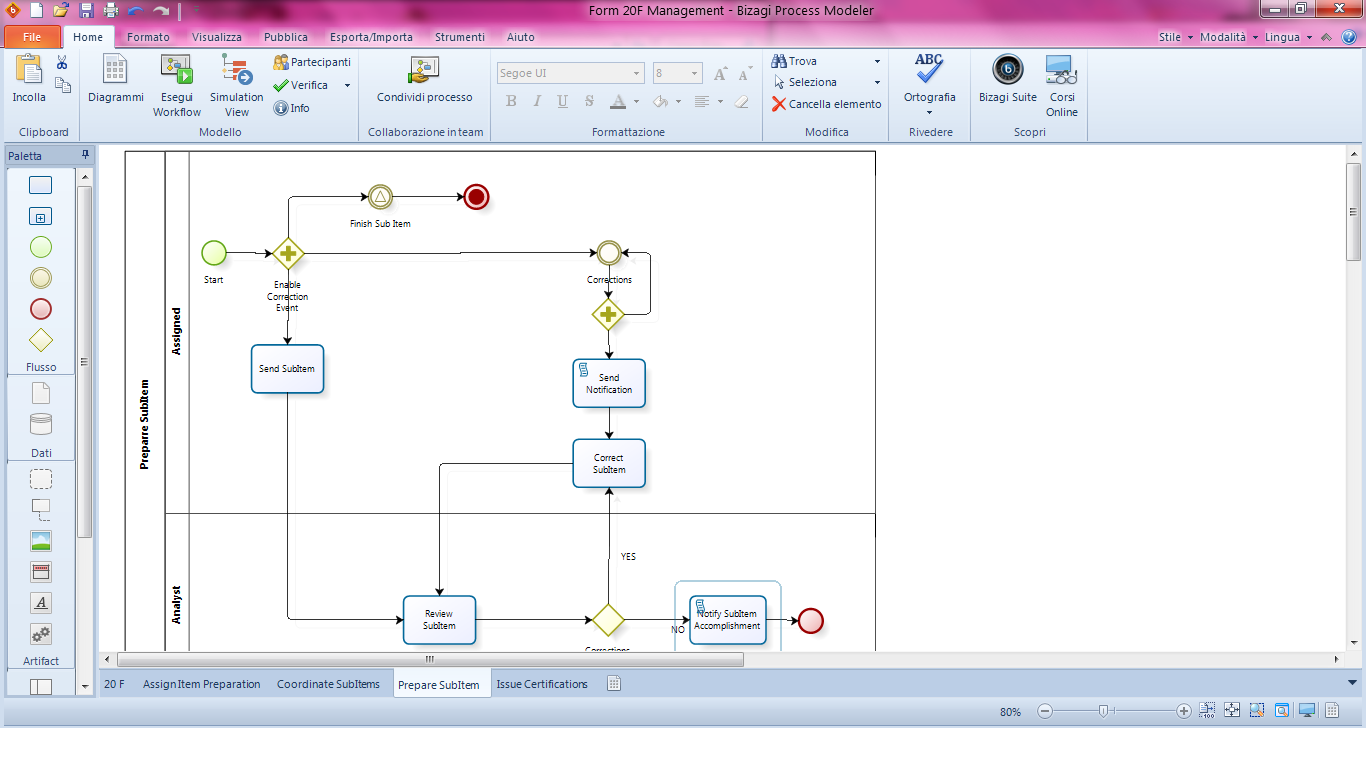
\includegraphics[width=\textwidth]{diagramma_biz}
\end{figure}
}
\end{columns}

\bigskip

\begin{columns}
\column{.5\textwidth}{
\begin{tabular}{m{.2\textwidth}m{.8\textwidth}}

\includegraphics[width=.13\textwidth]{biz_suite_logo} & Bizagi BPM Suite\\

\includegraphics[width=.13\textwidth]{biz_modeler_logo} & Bizagi Modeler\\
\end{tabular}
}
\column{.5\textwidth}{
\begin{alertblock}{\ding{56} Svantaggi:}
\begin{itemize}
  \item localizzazione incompleta
  \item simulazione carente
  \item interfaccia non intuitiva
\end{itemize}
\end{alertblock}
}
\end{columns}
\end{frame}

\renewcommand{\progname}{ProcessMaker}
\begin{frame}% #12
\frametitle{Una terza soluzione (PM)}
\begin{columns}
\column{.5\textwidth}{
\begin{figure}
  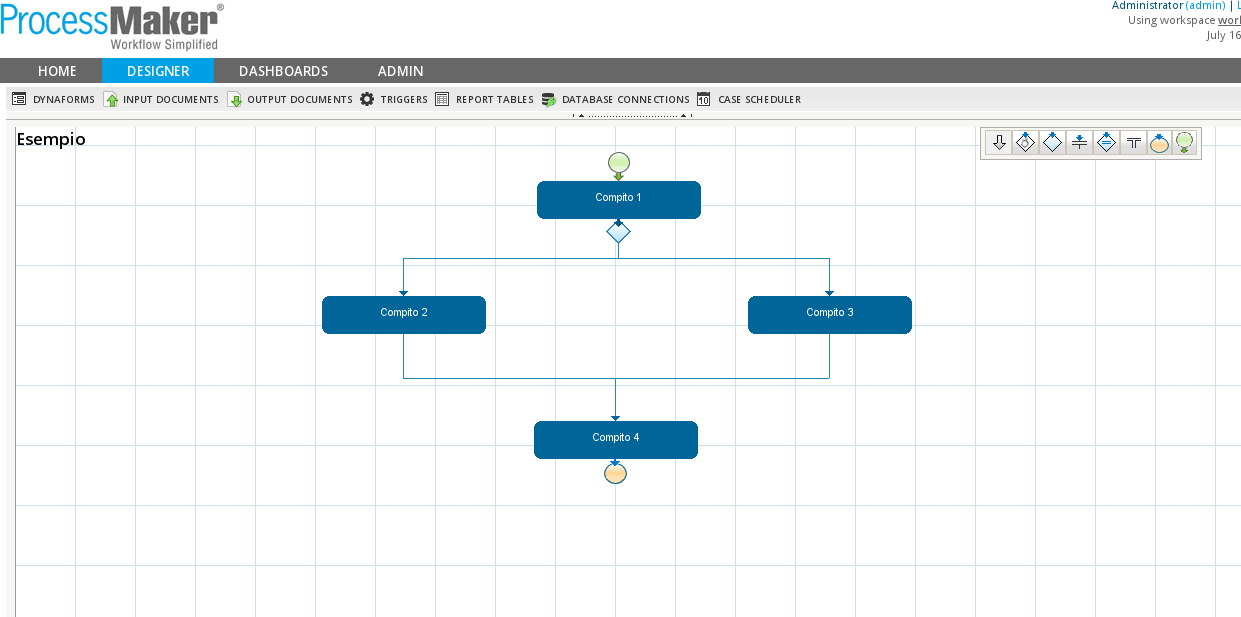
\includegraphics[width=\textwidth]{pm_editor}
\end{figure}
}
\column{.5\textwidth}{
\begin{exampleblock}{\ding{52} Vantaggi:}
\begin{itemize}
  \item piattaforma AMP
  \item servizi esterni \\(DBMS, email, LDAP)
  \item indicatori visuali avanzamento
  \item supporto della community
  \item form dinamici
\end{itemize}
\end{exampleblock}
}
\end{columns}

\begin{columns}
\column{.5\textwidth}{
\begin{alertblock}{\ding{56} Svantaggi:}
\begin{itemize}
  \item editor difficile da usare
  \item modellazione non standard
  \item configurazione complessa
  \item localizzazione incompleta
\end{itemize}
\end{alertblock}
}
\column{.5\textwidth}{
\begin{figure}
  
\includegraphics[width=.6\textwidth]{processmaker_logo}
\end{figure}
}
\end{columns}
\end{frame}

\renewcommand{\progname}{Camunda}
\begin{frame}% #14
\frametitle{Un approccio un po' diverso\ldots (Camunda)}
\begin{columns}
\column{.5\textwidth}{
\begin{figure}
  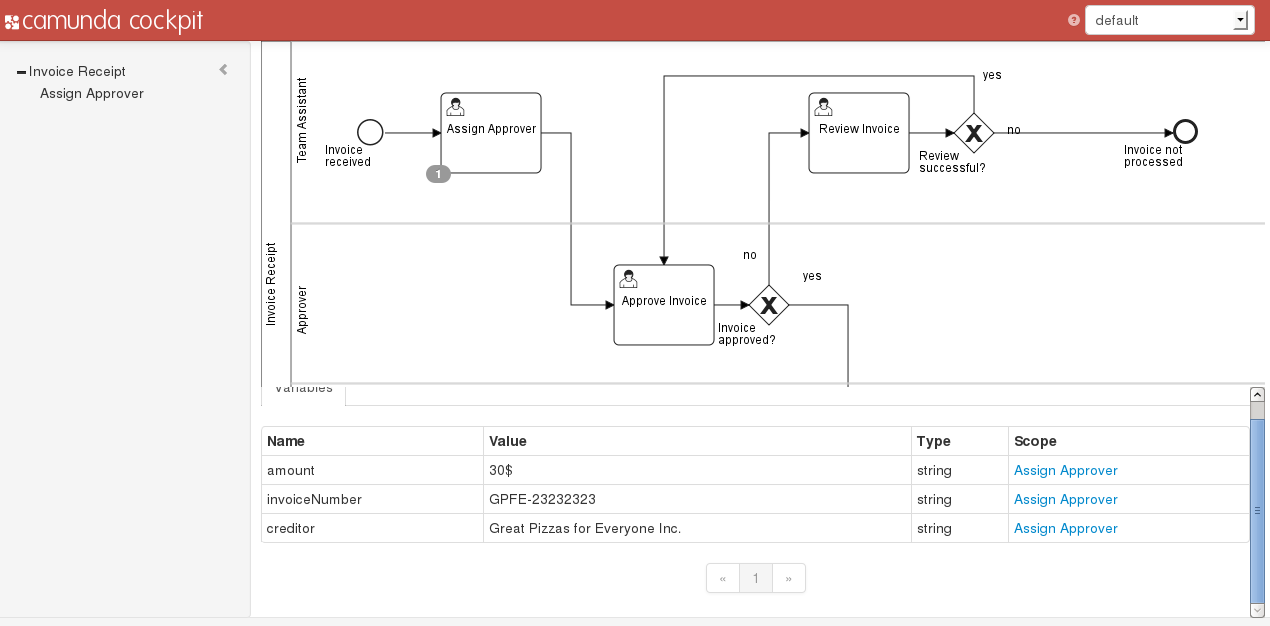
\includegraphics[width=\textwidth]{camunda_cockpit}
\end{figure}
}
\column{.5\textwidth}{
\begin{exampleblock}{\ding{52} Vantaggi:}
\begin{itemize}
  \item front-end modulari
  \item connettori per strumenti esterni
  \item cockpit di monitoraggio
  \item installazione facilitata
\end{itemize}
\end{exampleblock}
}
\end{columns}

\begin{columns}
\column{.5\textwidth}{
\begin{alertblock}{\ding{56} Svantaggi:}
\begin{itemize}
  \item non integra alcun editor
  \item no assistente per form
  \item complessa gestione (Cycle)
\end{itemize}
\end{alertblock}
}
\column{.5\textwidth}{
\begin{figure}
  
\includegraphics[width=.6\textwidth]{camunda_logo}
\end{figure}
}
\end{columns}
\end{frame}

\subsection{Analisi comparativa}
\begin{frame}% #15
\frametitle{Confronto fra le funzionalità delle soluzioni}
\begin{columns}
\column{.25\textwidth}{
\begin{figure}
  
\includegraphics[width=.9\textwidth]{test}
\end{figure}
}
\column{.75\textwidth}{
\scalebox{.65}{
\begin{tabular}{>{\sffamily}p{.75\textwidth}*{4}{>{\sffamily}c}}
\toprule
\bfseries{}Funzionalità & \bfseries{}BOS & \bfseries{}PM & \bfseries{}Bizagi & \bfseries{}Camunda\\
\midrule
modellazione                                  & \tick  & \tick  & \tick  & \cross \\
modellazione tramite \inglese{editor} grafico & \tick  & \tick  & \tick  & \cross \\
rispetto notazione BPMN                       & \tick  & \cross & \tick  & \cross \\
importazione/esportazione file XPDL           & \tick  & \tick  & \tick  & \cross \\
riutilizzo processi da adattare               & \tick  & \tick  & \tick  & \tick  \\
\inglese{template} di processi                & \tick  & \tick  & \tick  & \tick  \\
monitoraggio attività di processo (BAM)       & \tick  & \tick  & \tick  & \tick  \\
sistema di \inglese{reporting}                & \tick  & \tick  & \tick  & \tick  \\
indicatori grafici stato di avanzamento       & \cross & \tick  & \cross & \cross \\
ottimizzazione dei processi                   & \tick  & \cross & \cross & \cross \\
simulazione                                   & \tick  & \cross & \tick  & \cross \\
sistema di \inglese{reporting} simulazione    & \tick  & \cross & \tick  & \cross \\
validazione modelli                           & \tick  & \cross & \tick  & \cross \\
esecuzione automatizzata processi             & \tick  & \tick  & \tick  & \tick  \\
integrazione con \sw di parti terze           & \tick  & \tick  & \tick  & \tick  \\
interfacciamento con utenti                   & \tick  & \tick  & \tick  & \tick  \\
\inglese{form} statici                        & \tick  & \tick  & \tick  & \cross \\
\inglese{form} dinamici                       & \tick  & \tick  & \cross & \cross \\
\inglese{form} internazionalizzabili          & \tick  & \cross & \cross & \cross \\
gestione separata dei ruoli                   & \tick  & \cross & \cross & \tick  \\
usabilità                                     & \tick  & \tick  & \tick  & \tick  \\
facilità di installazione                     & \cross & \cross & \cross & \tick  \\
facilità di apprendimento                     & \cross & \cross & \cross & \cross \\
facilità utilizzo del \inglese{designer}      & \tick  & \cross & \cross & n.\,p. \\
disponibilità di documentazione               & \tick  & \tick  & \tick  & \tick  \\
multipiattaforma                              & \tick  & \tick  & \cross & \tick  \\
\bottomrule 
\end{tabular}
}
}
\end{columns}
\end{frame}

\section{Proposta di soluzione}
\begin{frame}% #16
\frametitle{La proposta di EBS}
\begin{columns}
\column{.5\textwidth}{
\begin{block}{Motivazioni}
\begin{itemize}
  \item potente e completo
  \item OSS (espandibile a pagamento)
  \item rispetto degli standard
  \item grande numero di connettori\tikz \coordinate (conn);
  \item report e ottimizzazione
  \item separazione dei ruoli
  \item creazione form semplificata
\end{itemize}
\end{block}
}
\column{.5\textwidth}{
\begin{figure}
  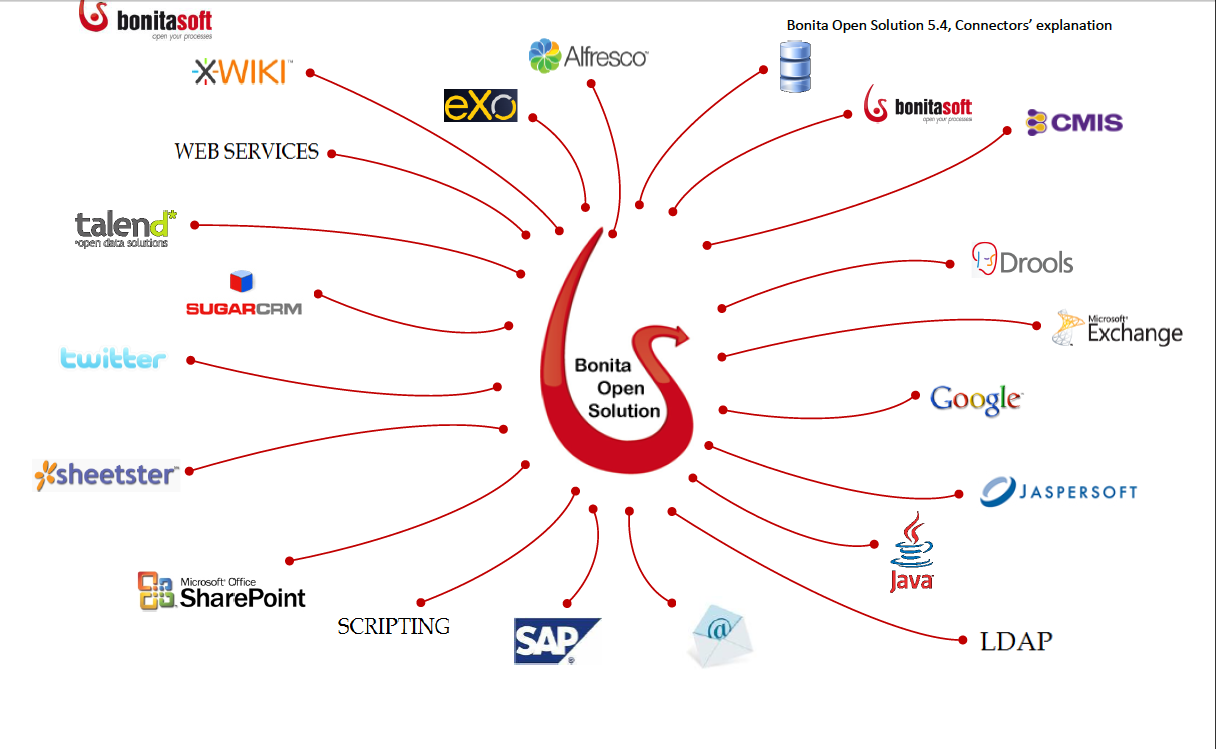
\includegraphics[width=\textwidth]{bosconnectors}
\end{figure}
}
\end{columns}

\begin{columns}
\column{.5\textwidth}{
\begin{exampleblock}<2->{Consuntivo:}
\begin{itemize}
  \item no manuale d'uso (doc online)
  \item no soluzione ibrida / ad hoc
\end{itemize}
\end{exampleblock}
}
\column{.5\textwidth}{
\uncover<2->{
\rotatebox{10}{\begin{tikzpicture}
\node at (0, 0) {
Costo totale: \EUR{4.915}
};
\draw[thick, red] (-1.5, -.3) -- ++(3, .5);
\draw[thick, red] (-1.5, .2) -- ++(3, -.5);
\node at (2, -1) {\Huge
\rotatebox{-10}{\textcolor{green}{\EUR{4.855}!}}
};
\end{tikzpicture}}
}
}
\end{columns}
\end{frame}

\begin{frame}
\frametitle{Una dimostrazione pratica\ldots}
\movie[showcontrols=true,width=.7\textwidth]{BOS}{tutorial.ogg}
\end{frame}
\end{document}
